% !TEX TS-program = xelatex
% !TEX encoding = UTF-8
\documentclass{QHUthesis}
\graphicspath{{figures/}}

\begin{document}
	%=====前言部分,封皮页需要自己填写的内容
	\frontmatter
	\title{{青海大学青海大学某某某某某某某某某某某某某某设计}}%中文标题
	\entitle{{QHU QHU QHU Design of bla bla bla bla bla bla bla bla bla bla}}%英文标题
	\author{WuZhiPeng}%论文作者
	\major{机械设计制造及其自动化}%专业、年级
	\advisor{某某某}%指导老师
	\college{机械工程学院}%学院
	\serialnumber{17000000000}%学号
	\cptdate{2021年5月20日}
	\stryear{2017级}%年级
	\captionsetup[figure][bi-second]{name=Fig} %设置图的英文编号前缀
	\captionsetup[table][bi-second]{name=Table} %设置表的英文编号前缀
	
%%======生成封面
\maketitle
\thispagestyle{empty} 
\newblankpage%插入一个新的空白页
%插入诚信责任书页面
\begin{center}
\heiti\zihao{-2}诚信责任书
\end{center}
\vspace{1cm}

\songti\zihao{4}本人郑重声明:本人所呈交的毕业论文(设计),是在导师的指导下独立进行研究所取得的成果。毕业论文(设计)中凡引用他人已经发表或未发表的成果、数据、观点等,均已明确注明出处。除文中已经注明引用的内容外,不包含任何其他个人或集体已经发表或在网上发表的论文。

特此声明。
\vspace{4cm}


\begin{flushleft}
论文作者签名:\QHUunderline[60pt]{}
\end{flushleft}

\begin{flushright}
日期:\QHUunderline[120pt]{}
\end{flushright}


\clearpage
\newblankpage%插入一个新的空白页
\clearpage
%======生成目录
\thispagestyle{empty} 
\tableofcontents
\thispagestyle {empty}

%方法3
%\newpage
%\pagestyle{empty}
%\tableofcontents
%\newpage
%\pagestyle{fancy}
%\setcounter{page}{1} %new page

\ifthenelse{\boolean{PicAndTabIndex}}
{
	\renewcommand{\listfigurename}{插图索引}
	\renewcommand{\listtablename}{附表索引}
	\setcounter{lofdepth}{1}
	\newcommand{\loflabel}{图~}
	\renewcommand{\numberline}[1]{\songti\zihao{4}\loflabel~#1\hspace*{\baselineskip}}
	\addcontentsline{toc}{chapter}{插图索引}
	\listoffigures
	\newcommand{\lotlabel}{表~}
	\renewcommand{\numberline}[1]{\songti\zihao{4}\lotlabel~#1\hspace*{\baselineskip}}
	\addcontentsline{toc}{chapter}{附表索引}
	\listoftables
}
{
}
%======文章主体
\mainmatter %开启章节序号计数,重置页码,页码使用阿拉伯数字;
\songti\zihao{-4} %正文字体为小四号宋体
% !TEX encoding = UTF-8
%======中文摘要内容格式:{中文摘要}{关键词}
\ZhAbstract{
青海大学(Qinghai University),位于青海省西宁市,是一所以工、农、医、管四大学科为主,其他学科协调发展的教学研究型大学,国家“双一流”建设高校,国家“211工程”重点建设大学,是清华大学等6所知名高校的对口支援学校,是全国14所“中西部高校提升综合实力”工程入选高校,国家首批百所创新示范校,教育部与青海省人民政府部省合建高校,具有学士、硕士、博士学位授予权。

学校前身为青海工学院,始建于1958年。1960年11月,与青海农牧学院、青海医学院、青海财经学院合并为青海大学,“文革”初期被撤销。1971年恢复青海工农学院,设有工、农两大学科。1988年恢复青海大学。1997年10月,青海畜牧兽医学院并入青海大学。2001年1月,青海省农林科学院、青海省畜牧兽医科学院、青海财经职业学院整建制划归青海大学,2004年青海医学院并入,组建成新的青海大学。

截至2022年1月,学校占地3000余亩;有本科专业67个,博士后科研流动站1个,一级学科博士学位授权点5个,一级学科硕士学位授权点20个,交叉学科硕士学位授权点1个,二级学科硕士学位授权点共计108个;有硕士专业学位授权类别15个,共计96个专业领域;有教职工5356人(含附属医院3054人),专任教师1451人,在校生2.5万余人,其中研究生3714人、本专科生1.9万余人(含昆仑学院3838人)。}{青海大学;211大学;双一流建设高校}
%======中文摘要内容格式:{英文摘要}{关键词}
\EnAbstract{
Qinghai University, located in Xining City, Qinghai Province, is a teaching and research university with four major disciplines: engineering, agriculture, medicine and management, and coordinated development of other disciplines. "It is also one of the 14 universities selected for the project of "Midwest Universities to Improve Comprehensive Strength", the first batch of 100 innovative demonstration universities, and the university jointly built by the Ministry of Education and Qinghai Provincial People's Government, with the right to confer bachelor, master and doctoral degrees. It has the right to confer bachelor, master and doctoral degrees.
	
In November 1960, it was merged with Qinghai Agricultural and Animal Husbandry College, Qinghai Medical College and Qinghai Finance and Economics College to form Qinghai University, which was abolished at the beginning of the Cultural Revolution. 1971, Qinghai Agricultural and Industrial College was restored, with two major disciplines of engineering and agriculture, and Qinghai University was restored in 1988. In October 1997, Qinghai College of Animal Husbandry and Veterinary Medicine was incorporated into Qinghai University, and in January 2001, Qinghai Academy of Agriculture and Forestry, Qinghai College of Animal Husbandry and Veterinary Medicine and Qinghai College of Finance and Economics were incorporated into Qinghai University, and in 2004, Qinghai College of Medicine was incorporated into Qinghai University.

As of January 2022, the university covers an area of more than 3,000 mu; there are 67 undergraduate programs, 1 postdoctoral research station, 5 authorized doctoral degree programs in primary disciplines, 20 authorized master's degree programs in primary disciplines, 1 authorized master's degree program in cross-disciplinary disciplines, and 108 authorized master's degree programs in secondary disciplines; there are 15 authorized master's degree categories with a total of 96 professional fields; there are There are 5,356 faculty members (including 3,054 in affiliated hospitals), 1,451 full-time teachers, and more than 25,000 students, including 3,714 postgraduates and 19,000 undergraduates (including 3,838 in Kunlun College).}{QHU; 211 project; Double First-Class Strategic Plan}%如果中英文摘要和目录一起罗马数字编页码,请把部分移到\mainmatter前
% !TEX encoding = UTF-8
%%=====自定义页眉页脚
%\pagestyle{fancy}
%\fancyhf{}
%\chead{这里是标题这里是标题这里是标题}

\renewcommand{\headrulewidth}{0.4pt} 
\chapter{青海大学 \LaTeX 模板}
\section{Why \LaTeX ? }
\LaTeX(LATEX,音译“拉泰赫”)是一种基于TEX的排版系统,由美国计算机学家莱斯利·兰伯特(Leslie Lamport)在20世纪80年代初期开发,利用这种格式,即使使用者没有排版和程序设计的知识也可以充分发挥由\TeX{}所提供的强大功能,能在几天,甚至几小时内生成很多具有书籍质量的印刷品。对于生成复杂表格和数学公式,这一点表现得尤为突出。因此它非常适用于生成高印刷质量的科技和数学类文档。这个系统同样适用于生成从简单的信件到完整书籍的所有其他种类的文档。

为了方便青海大学本科生将更多的时间集中于论文的内容当中,而不是在格式的调节上浪费时间。\LaTeX 提供了一个很好的方式。\LaTeX 具有很多优点就不说了,大家可以多用用。
\par 下文就是简单的版式,与青海大学毕业论文写作规范.doc中要求一致。若有不同请与我联系。

bla bla bla bla bla bla bla bla bla bla bla bla bla bla bla bla bla bla bla bla bla bla bla bla bla bla bla bla bla bla bla bla bla bla bla bla bla bla bla bla bla bla bla bla bla bla bla bla bla bla bla bla bla bla bla bla bla bla bla bla bla bla bla bla bla bla bla bla bla bla bla bla bla bla bla bla bla bla bla bla bla bla bla bla bla bla bla bla bla bla

\subsection{选题背景与意义(四号仿宋)}
主要介绍毕业设计选题的背景及为什么要做这个事,即这个事的意义。为了便于操作,可以先把文字复制到写字板后,再粘贴到相应位置,格式会保持不变。
\subsection{国内外研究现状}
主要介绍国内与国外在这个选题方面的研究情况、进展及存在的问题,也就顺势引入你做这个选题的意义了(可以解决存在的问题)。这部分可以分国内、国外两个小节来介绍,也可以不分小节来讲。这部分引用别人的研究成果的较多,一定要进行标注,并在参考文献中按出现顺序进行一一列举出来。凡引用、转述、参考他人的成果或资料,均须注明出处。
\subsubsection{国内研究现状}
主要是国内在这方面的研究情况、进展与存在的问题。
\subsubsection{国外研究现状}
主要是国外在这方面的研究情况、进展与存在的问题。
 %各个章节内容单独分开撰写,方便编译和组织;
% !TEX encoding = UTF-8

\chapter{我是一级标题}
论文正文中各标题要突出重点、简明扼要。字数一般在15字以内,不得使用标点符号。标题中尽量不采用英文缩写词,对必须采用者,应使用本学科的通用缩写词。

我是正文内容,我是正文内容,我是正文内容,我是正文内容,我是正文内容,我是正文内容,我是正文内容,我是正文内容,我是正文内容,我是正文内容,我是正文内容,我是正文内容,我是正文内容,我是正文内容,我是正文内容,我是正文内容,我是正文内容,我是正文内容,我是正文内容,我是正文内容,我是正文内容,我是正文内容,我是正文内容,我是正文内容,我是正文内容,我是正文内容,我是正文内容,我是正文内容,我是正文内容,我是正文内容,我是正文内容,我是正文内容,我是正文内容,我是正文内容,我是正文内容,我是正文内容,我是正文内容,我是正文内容,我是正文内容,我是正文内容,我是正文内容,我是正文内容,我是正文内容,我是正文内容,我是正文内容,我是正文内容,我是正文内容,我是正文内容,我是正文内容,我是正文内容,我是正文内容,我是正文内容,我是正文内容,我是正文内容,我是正文内容,我是正文内容,我是正文内容,我是正文内容,我是正文内容,我是正文内容,我是正文内容,我是正文内容,我是正文内容,我是正文内容,我是正文内容,我是正文内容,我是正文内容,我是正文内容,我是正文内容,我是正文内容,我是正文内容,我是正文内容,我是正文内容,我是正文内容,我是正文内容,我是正文内容,我是正文内容,我是正文内容,我是正文内容,我是正文内容,我是正文内容,我是正文内容,我是正文内容,我是正文内容,我是正文内容,我是正文内容,我是正文内容,我是正文内容,我是正文内容,我是正文内容,我是正文内容,我是正文内容,我是正文内容,我是正文内容,我是正文内容,我是正文内容,我是正文内容,我是正文内容,我是正文内容,我是正文内容,我是正文内容,我是正文内容,我是正文内容,我是正文内容,我是正文内容,我是正文内容,我是正文内容,我是正文内容,我是正文内容,我是正文内容,我是正文内容,我是正文内容,我是正文内容,我是正文内容,我是正文内容,我是正文内容,我是正文内容,我是正文内容,我是正文内容,我是正文内容,我是正文内容。
\section{我是二级标题}
系统用户主要分为买家用户与卖家用户,在系统中通过注册并登陆后,用户可以以买家的身份浏览已发布的商品并进行购买;用户如需出售二手物品,可在系统中进行发布商品,同时用户也变为卖家的身份,即人人都是买家,人人也都是卖家。
\subsection{我是三级标题}
根据系统用例图,卖家主要对商品进行出售的操作,根据操作流程可分为:发布商品、管理商品和出售商品三个功能。
% !TEX encoding = UTF-8

\chapter{系统配置}
正确编译需要以下几个部分(这是一个列表环境):
\begin{itemize}
\item 一个基本的TEX发行版
\item CJK或XeCJK(供\LaTeX{})宏包
\item ctex宏包(提供ctexbook文档).
\item 中文字体
\item 如果要使用 biblatex 进行文献列表和引用的排版的话, 还需要 biblatex 宏包。
\end{itemize}
% !TEX encoding = UTF-8
\chapter{模板使用}
\section{模板文件结构\label{sec:files}}
整个模板根目录的文件列表如下:
\begin{center}
\begin{tabular}{|l|l|l|}
\hline
QHUthesis.cls & ---QHUthesis宏包 & \textcolor{red}{{*}}\\
\hline
QHU.cfg & ---QHU宏包配置文件 & \textcolor{red}{{*}}\\
\hline
QHUbib.bst & ---引文样式文件 & \textcolor{red}{{*}}\\
\hline
references/reference.bib & ---bib数据库 & \textcolor{red}{{*}}\\
\hline
figures/QHUbmp.bmp & ---青海大学校名标准字 & \textcolor{red}{{*}}\\
\hline
QHUbachelor.tex & ---\TeX{}样例文件 &\textcolor{red}{{*}}\\
\hline
\end{tabular}
\end{center}
注: \textcolor{red}{{*}} 表示\LaTeX{}模板必须的文件。
\section{示例}
对于论文中最常使用的一些功能在本节中给出示例。
\subsection{公式}
\begin{equation}
\hat{H}=\frac{\epsilon}{2}\hat{\sigma}_{z}-\frac{\Delta}{2}\hat{\sigma}_{x}+\sum_{k}\omega_{k}\hat{b}_{k}^{\dagger}\hat{b}_{k}+\sum_{k}\frac{g_{k}}{2}\hat{\sigma}_{z}(\hat{b}_{k}+\hat{b}_{k}^{\dagger})\label{eq:sbm}
\end{equation}
根据公式\ref{eq:sbm}可知,这个是对公示的引用。
\begin{align}\label{eqn3:9}
\int_{-\infty}^{+\infty}S(\tau,f)\,\mathrm{d}\tau&=\int_{-\infty}^{+\infty}x(t)\left\{\int_{-\infty}^{+\infty}\frac{|f|}{\sqrt{2\pi}}e^{\frac{-|f|^2(\tau-t)^2}{2}}\,\mathrm{d}\tau\right\}e^{-j2\pi ft}\,\mathrm{d}t\notag\\
&=\int_{-\infty}^{+\infty}x(t)e^{-j2\pi ft}\left\{\int_{-\infty}^{+\infty}\frac{1}{\sqrt{\pi}}e^{-\left[\frac{|f|(\tau-t)}{\sqrt{2}}\right]^2}\,\mathrm{d}\frac{|f|(\tau-t)}{\sqrt{2}}\right\}\,\mathrm{d}t
\end{align}
令$\theta=\frac{|f|(\tau-t)}{\sqrt{2}}$,则式\eqref{eqn3:9}可改写为
\begin{align}\label{eqn3:10}
\int_{-\infty}^{+\infty}S(\tau,f)\,\mathrm{d}\tau&=\int_{-\infty}^{+\infty}x(t)e^{-j2\pi ft}\,\mathrm{d}t\frac{1}{\sqrt{\pi}}\int_{-\infty}^{+\infty}e^{-\theta^2}\,\mathrm{d}\theta\notag\\
&=\int_{-\infty}^{+\infty}x(t)e^{-j2\pi ft}\,\mathrm{d}t\frac{2}{\sqrt{\pi}}\int_{0}^{+\infty}e^{-\theta^2}\,\mathrm{d}\theta\notag\\
&=\int_{-\infty}^{+\infty}x(t)e^{-j2\pi ft}\,\mathrm{d}t\notag\\
&=X(f)
\end{align}
\subsection{表格}
\begin{table}[H]
	\begin{center}
		\caption{希腊字母表\label{tab:Greek}}
		\begin{tabular}{|c|c|c|c|c|}
			\hline
			Alpha & Beta & Gamma & Delta & Theta\\
			\hline
			$\alpha$ & $\beta$ & $\gamma$ & $\delta$ & $\theta$\\
			\hline
			$A$ & $B$ & $\Gamma$ & $\Delta$ & $\Theta$\\
			\hline
		\end{tabular}
		\end{center}
\end{table}
这是对表\ref{tab:Greek}的引用

\begin{table}[htbp]
	\caption{不同电力系统频率测量算法时间复杂度比较}\label{table2:1}
	\centering\zihao{5}
	\begin{tabular}{cccc}
		\toprule[1.5pt]
		算法 &  加法 & 乘法 & 时间复杂度 \\
		\midrule[1pt]
		TQDS       & $QN^2+QN/2+Q+1$        &$QN^2$                      & $O(N^2)$     \\
		WIFFT         & $(QN+1)\log_2(QN+1)$ & $(QN+1)*(1+\log_2(QN+1))$ &$O(N\log_2N)$\\
		本章算法 &$3(QN+1)\log_2(QN+1)$    & $(QN+1)(1+3\log_2(QN+1))$          & $O(N\log_2N)$\\
		\bottomrule[1.5pt]
	\end{tabular}
	\vspace{\baselineskip}
\end{table}

本章对时域准同步算法(Time Domain Quasi-synchronous,TQDS)、加窗插值~FFT~算法(Windowed Interpolated FFT,WIFFT)以及本章所提算法的时间复杂度进行分析。因~TQDS~需要进行迭代运算,故设总采样点数为~$QN+1$,其中~$Q$~为迭代次数,$N$~为单次迭代所需的数据点长度。TQDS~共需要~$QN^2$~次加法和~$QN^2+QN/2+Q+1$~次乘法,因此~TQDS~的时间复杂度为~$O(N^2)$。WIFFT~的计算量主要为~FFT~运算,共需进行~$(QN+1)\log_2(QN+1)$~次加法和~$(QN+1)(1+\log_2(QN+1))$~次乘法,因此~WIFFT~的时间复杂度为~$O(N\log_2N)$。对于本章所提出的算法,由于线性卷积运算采用快速卷积来进行计算,因此共需进行~$3(QN+1)\log_2(QN+1)$~加法和~$(QN+1)(1+3\log_2(QN+1))$~次乘法,算法时间复杂度为~$O(N\log_2N)$。表~\ref{table2:1}~对三种频率测量算法的时间复杂度进行了对比。由表~\ref{table2:1}~可见,TQDS~的时间复杂度比其它两种算法要高,本章算法和~WIFFT~时间复杂度相当,有利于算法的实时实现。
\subsection{图形}
这个示例为插入图片:
\begin{figure}[H]
	\centering
		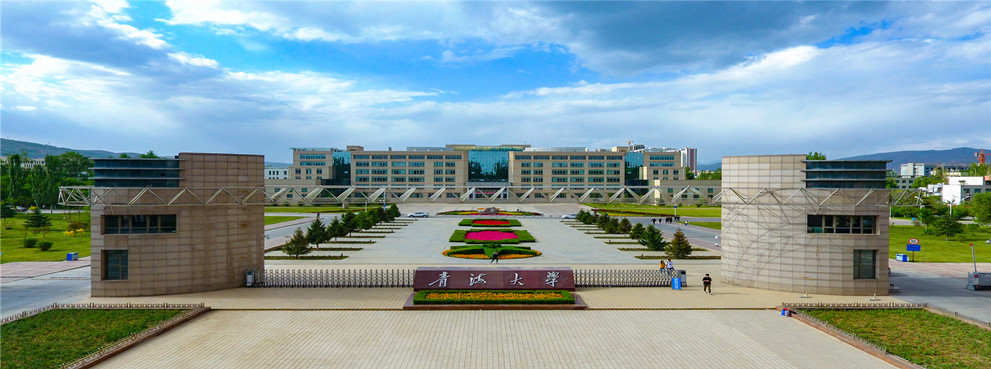
\includegraphics[width=0.618\textwidth]{figure.jpg}%图片名称,放在/figures目录下
	\caption{图片插入\label{fig:fig}}
\end{figure}
具体代码:
\begin{verbatim}%抄写环境
\begin{figure}[H]
\centering
%图片放在/figures目录下
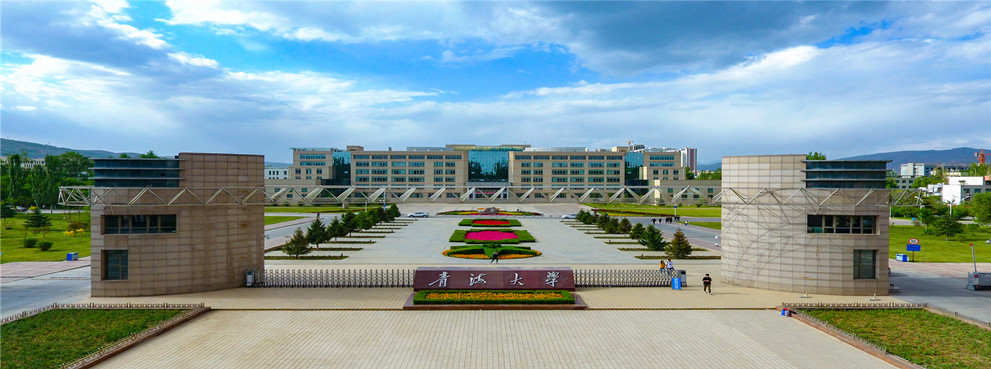
\includegraphics[width=0.618\textwidth]{figure.jpg}
\caption{图片插入\label{fig:fig}}
\end{figure}
\end{verbatim}
\begin{figure}[H]
\centering
		
\includegraphics[width=0.618\textwidth]{QHU.bmp}
\caption{青海大学\label{fig:qhu}}
\end{figure}
对于图\ref{fig:fig}和图\ref{fig:qhu}的引用。
\subsection{引用}
\subsubsection{交叉引用}
对所有需要引用的公式、表格、图形,执行插入--标签后,即可使用插入-- 交叉引用自动产生引用。
\begin{itemize}
\item 哈密顿量见方程~\eqref{eq:sbm}。
\item 希腊字母表见表~\ref{tab:Greek}。引用格式与方程引用格式不同
\item 校名标准字如图~\ref{fig:qhu}。 引用格式与方程引用格式不同
\end{itemize}
具体见代码:
\begin{verbatim}
\begin{itemize}
\item 哈密顿量见方程~\eqref{eq:sbm}。
\item 希腊字母表见表~\ref{tab:Greek}。引用格式与方程引用格式不同
\item 校名标准字如图~\ref{fig:qhu}。 引用格式与方程引用格式不同
\end{itemize}
\end{verbatim}
\subsubsection{文献引用}
将引文的bib数据库(默认文件名为reference.bib)放入模板根目录下的references文件夹,即可通过插入--文献引用自动产生引文。
\begin{itemize}
\item Journal:An article \cite{ELIDRISSI94,MELLINGER96,SHELL02,cnarticle}。
\item Book:An book \cite{IEEE-1363,tex,companion}。
\item Conference:A conference \cite{kocher99,DPMG,cnproceed}。
\item Manual:A manual\cite{NPB2}.
\item MasterThesis:\cite{zhubajie,metamori2004,shaheshang,FistSystem01}.
\end{itemize}
\subsection{伪代码实现}
\begin{algorithm}
\caption{放进冰箱的大象}\label{算法实例}
\begin{algorithmic}
	\REQUIRE 有一只大象
	\ENSURE 放进冰箱里
	\FOR {没有剩余的大象}
	\IF {大象比冰箱大}
	\STATE 把大象分割
	\ENDIF
	\ENDFOR
	\STATE 第一步
	\STATE 第二步
	\STATE 第三步
\end{algorithmic}
AAA\end{algorithm}
\subsection{代码展示}
可以把你的程序添加到附录里,展示自己的工作。
\begin{lstlisting}[language={[ANSI]C}, numbers=left]
#include <stdio.h>
int main(int argc, char ** argv)
{
/*打印Hello,world*/
printf("Hello, world!\n");

return 0;
}
\end{lstlisting}
\section{依赖}
QHUthesis依赖于以下宏包,这些宏包在常见的\LaTeX{}发行版中都包括,在安装使用之前,请确定你的\TeX{}发行版中都已正常安装这些宏包
\begin{table}[H]
	\centering
	\begin{tabular}{cccc}
		\hline
		{footmisc} &  {amsmath} &  {amsfonts} &  {amssymb} \\
		
		{graphicx} &  {svgnames} &  {xcolor} &  {mathptmx} \\
		
		{float} &  {fontenc} &  {fancyhdr} &  {lastpage} \\
		
		{etoolbox} &  {fancy} &  {caption} &  {array} \\
		
		{makecell} &  {forloop} &  {xstring} &  {hyperref} \\
		
		{tabularx} &  {enumitem} &  {ntheorem} &  {algorithm}\\
		
		{algorithmic} &  {bibentry} &  {xeCJK} &  {CJK} \\
		{listings} &  {courier} &  {} &  {} \\
		\hline
	\end{tabular}
\end{table}
如果你尚未安装这些宏包,可以启动你的 \TeX{} 发行版的宏包管理器
来安装;或者到 \url{http://www.ctan.org} 上搜索下载并安装。
\section{基本设置}
\begin{enumerate}
	\item 图片搜索路径默认设置为模板根目录下的figures/。
	\item bib数据库默认设置为模板根目录下的references/reference.bib。 其中bib文件可由任意文献库管理软件自动生成
\end{enumerate}


% !TEX encoding = UTF-8

\chapter{简单帮助}
\section{文字命令}
\subsection{常用命令}
\LaTeX 提供了一系列命令,用于修改字体、字号、数字等的呈现形式。

本论文中字体如下:
\subsubsection{字体}
\begin{verbatim}
宋体: \songti    启用宋体。
黑体: \heiti     启用黑体。
仿宋: \fangsong  启用仿宋。
楷书: \kaishu    启用楷书。
\end{verbatim}
{\songti 宋体} {\heiti 黑体}    {\fangsong 仿宋}     {\kaishu 楷书}
\subsubsection{字号}%
\begin{center}
	\begin{tabular}{cccccccc}
		\toprule
		初号 & 小初 & 一号 & 小一 & 二号 & 小二 & 三号 & 小三 \\
		0 & -0 & 1 & -1 & 2 & -2 & 3 & -3 \\
		\hline
		四号 & 小四 & 五号 & 小五 & 六号 & 小六 & 七号 & 八号 \\
		4 & -4 & 5 & -5 & 6 & -6 & 7 & 8 \\
		\bottomrule
	\end{tabular}
\end{center}
{\zihao{0}初号}; \dots {\zihao{4}四号};\dots \zihao{7}{七号}

%=======论文后部=======
\backmatter
%=======参考文献
\bibdatabase{references/reference}%参考文献数据库
\printbib%打印参考书目
% !TEX encoding = UTF-8
\Thanks
这里是致谢页,你可以在这里致谢你的父母,亲戚和朋友,勿忘我:),你们的指导老师。%致谢
\makeappedixfigtabnum%重新计算附图和表的标题号和计数号
% !TEX encoding = UTF-8
\Appendix
这里是附录页,附上你的程序或必要的相关知识

\bf\songti\color{red}{若要生成目录和参考文献的编译方式:} \color{black}XeLaTeX -->BibTeX --> XeLaTeX--> XeLaTeX

\songti
对于一些不宜放入正文中、但作为毕业论文(设计)又是不可缺少的部分,或有重要参考价值的内容,可编入毕业论文(设计)的附录中。例如,过长的公式推导、重复性的数据、图表、程序全文及其说明等。论文的附录依序用大写正体A,B,C……编序号,如:附录A。附录中的图、表、式等另行编序号,与正文分开,也一律用阿拉伯数字编码,但在数码前冠以附录序码,如:图A1;表B2;式(B3)等,

这个示例为插入图片:
\begin{figure}[H]
	\centering
	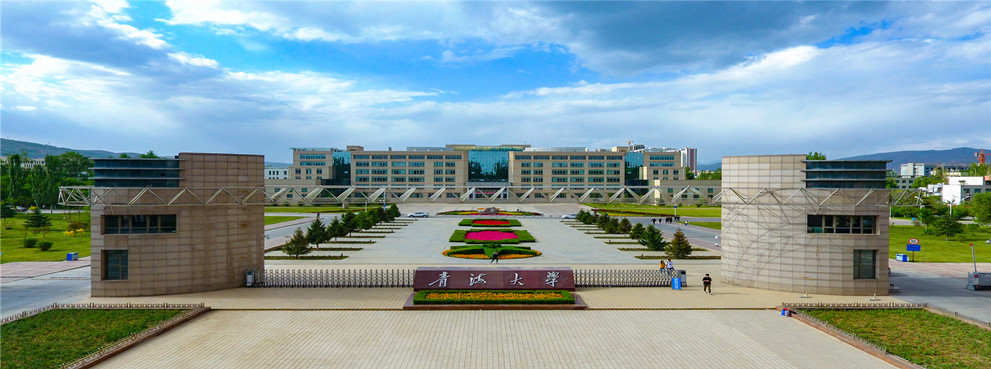
\includegraphics[width=0.618\textwidth]{figure.jpg}%图片名称,放在/figures目录下
	\caption{图片插入\label{fig:fig}}
\end{figure}%附录

\end{document}